%-------------------------------------------------------------------------------
%                                PREAMBLE
%-------------------------------------------------------------------------------
\documentclass[usenames,dvipsnames,svgnames,9pt]{beamer}
\usetheme{flow} % This theme uses TIKZ: compile twice with PDFLaTeX or LuaLaTeX.
%\cleanslidestrue

\usepackage{hyperref,graphicx,lmodern}
\usepackage[utf8]{inputenc}
\usepackage{tikz}
\usepackage{pgfplots}
\usepackage{xcolor}
\usepackage[makeroom]{cancel}
\usepackage{listings}
\usepackage{soul}

\graphicspath{{imgs/}}

\newenvironment{customlegend}[1][]{%
    \begingroup
    % inits/clears the lists (which might be populated from previous
    % axes):
    \csname pgfplots@init@cleared@structures\endcsname
    \pgfplotsset{#1}%
}{%
    % draws the legend:
    \csname pgfplots@createlegend\endcsname
    \endgroup
}%

\def\addlegendimage{\csname pgfplots@addlegendimage\endcsname}

%-------------------------------------------------------------------------------
%                                TITLE PAGE
%-------------------------------------------------------------------------------
\title[AMG solver for the coarse grid solve] % Short title used in footline
{
	AMG solver for the coarse grid solve % Long title
}

\author[Nicolas Offermans] % Presenting author in short form used in footline
{
	\underline{Nicolas Offermans}$^1$ \\
	Philipp Schlatter$^1$ \\
	Adam Peplinski$^1$ \\
	Oana Marin$^2$
}
% - Give the names in the same order as the appear in the paper.
% - Underline the presenting author.

\institute[unused]
{
	$^1$Linn\'e FLOW Centre, KTH Mechanics \\
	$^2$Argonne National Laboratory
}
% Keep it simple, no one is interested in your street address.

% University logo(s)
\logot{
\includegraphics[width=.105\paperwidth]{KTH-logo}}  % Top logo
\logob{
\includegraphics[width=.105\paperwidth]{Flow-logo}} % Bottom logo

\date[unused]
	{Nek Users meeting - 10 Aug. 2016}
% - Either use conference name or its abbreviation.
% - Not really informative to the audience, more for people (including
%   yourself) who are reading the slides online

% Uncomment this if you want the table of contents to pop up at the 
% beginning of each section (you can do the same with subsections):
%\AtBeginSection[]
%{
%  \begin{frame}<beamer>
%    \tableofcontents[currentsection,currentsubsection]
%  \end{frame} \addtocounter{framenumber}{-1}
%}

% If you wish to uncover everything in a step-wise fashion, uncomment
% the following command: 
% \beamerdefaultoverlayspecification{<+->}




\begin{document}

\titleframe % Print the title as the first slide


%------------------------------------------------
\section{Introduction}
%------------------------------------------------

\begin{frame}{Introduction}{}

\textbf{Outline:}

\begin{itemize}
\item Coarse grid solver
\vspace{5mm}
\item Parallelization of the AMG setup
\vspace{5mm}
\item My other projects
\end{itemize}

\end{frame}

\section{Coarse grid solver}

\begin{frame}{Coarse grid solver}{}

\begin{itemize}
\item Preconditioner for pressure operator: 
\begin{equation*}
M_0^{-1} := R_0 T_0^{-1} R_0^T + \sum_{k=1}^{K} R_k^T \tilde{T}_k^{-1} R_k.
\end{equation*}

\item Coarse grid part:
\begin{align*}
\Delta p & = r \\
\Leftrightarrow M_0^{-1} \Delta p & = M_0^{-1}r \\
\Leftrightarrow \underbrace{T_0^{-1}}_{A} \underbrace{R_0^T \Delta p}_{x} & = \underbrace{T_0^{-1} R_0^T r}_{b}
\end{align*}

\item Coarsening - Interpolation - Smoothing operators:
\begin{equation*}
 A = 
 \begin{bmatrix}
  A_{ff} & A_{fc} \\
  A_{cf} & A_{cc}
 \end{bmatrix}, \qquad
 P = 
 \begin{bmatrix}
  W \\
  I,
 \end{bmatrix}, \qquad
 B = 
 \begin{bmatrix}
  \hat{B}_{ff} &  \\
   & 0
 \end{bmatrix}.
\end{equation*}
\end{itemize}

Developed by J. Lottes.

\end{frame}

\section{AMG Setup}

\begin{frame}{AMG Setup}{Coarsening - Interpolation - Smoothing}

\begin{minipage}{0.48\linewidth}
\textbf{Coarsening} the mesh by defining different levels.

\onslide<4->{
\vspace{3mm}
\textbf{Interpolation operator:} 
\begin{itemize}
\item Between coarse and fine grids
\item Interpolation support
\item Interpolation weight
\end{itemize}
}
\onslide<5->{
\vspace{3mm}
\textbf{Smoothing} high frequency errors.
}
\end{minipage}
\begin{minipage}{0.03\linewidth}
\end{minipage}
\begin{minipage}{0.48\linewidth}
\begin{tikzpicture}
\draw[step=1.3cm,gray] (-2.6001,-2.6001) grid (2.6,2.6);
\only<1>{
\foreach [count=\x] \xc in {-2.6,-1.3,0,1.3,2.6}
	\foreach [count=\y] \yc in {-2.6,-1.3,0,1.3,2.6}
        \filldraw[red] (\xc, \yc) circle (1.5pt);
}
\only<2>{
\foreach [count=\x] \xc in {-2.6,-1.3,0,1.3,2.6}
	\foreach [count=\y] \yc in {-2.6,-1.3,0,1.3,2.6}
        \filldraw[red,opacity=0.5] (\xc, \yc) circle (1.5pt);
        
\foreach [count=\p] \pt in {(-1.3, 1.3),(1.3, 1.3),(-1.3, -1.3),(1.3, -1.3)}
        \filldraw[green] \pt circle (2pt);
}
\only<3->{
\foreach [count=\x] \xc in {-2.6,-1.3,0,1.3,2.6}
	\foreach [count=\y] \yc in {-2.6,-1.3,0,1.3,2.6}
        \filldraw[red,opacity=0.5] (\xc, \yc) circle (1.5pt);
        
\foreach [count=\p] \pt in {(-1.3, 1.3),(1.3, 1.3),(-1.3, -1.3),(1.3, -1.3)}
        \filldraw[green, opacity=0.5] \pt circle (2pt);
        
\filldraw[blue] (-1.3, 1.3) circle (2.5pt);
}
\end{tikzpicture}
\end{minipage}
\end{frame}

\section{Motivations}

\begin{frame}{Motivations for AMG}
\begin{itemize}
\item Efficiency of XXT limited when $(P,n) > (10^4, 10^5)$.
\item AMG is tunable.
\item Scaling tests results (Turbulent pipe - $Re_{\tau} = 550$ - {\color{red} XXT} - {\color{blue} AMG}).

\centering
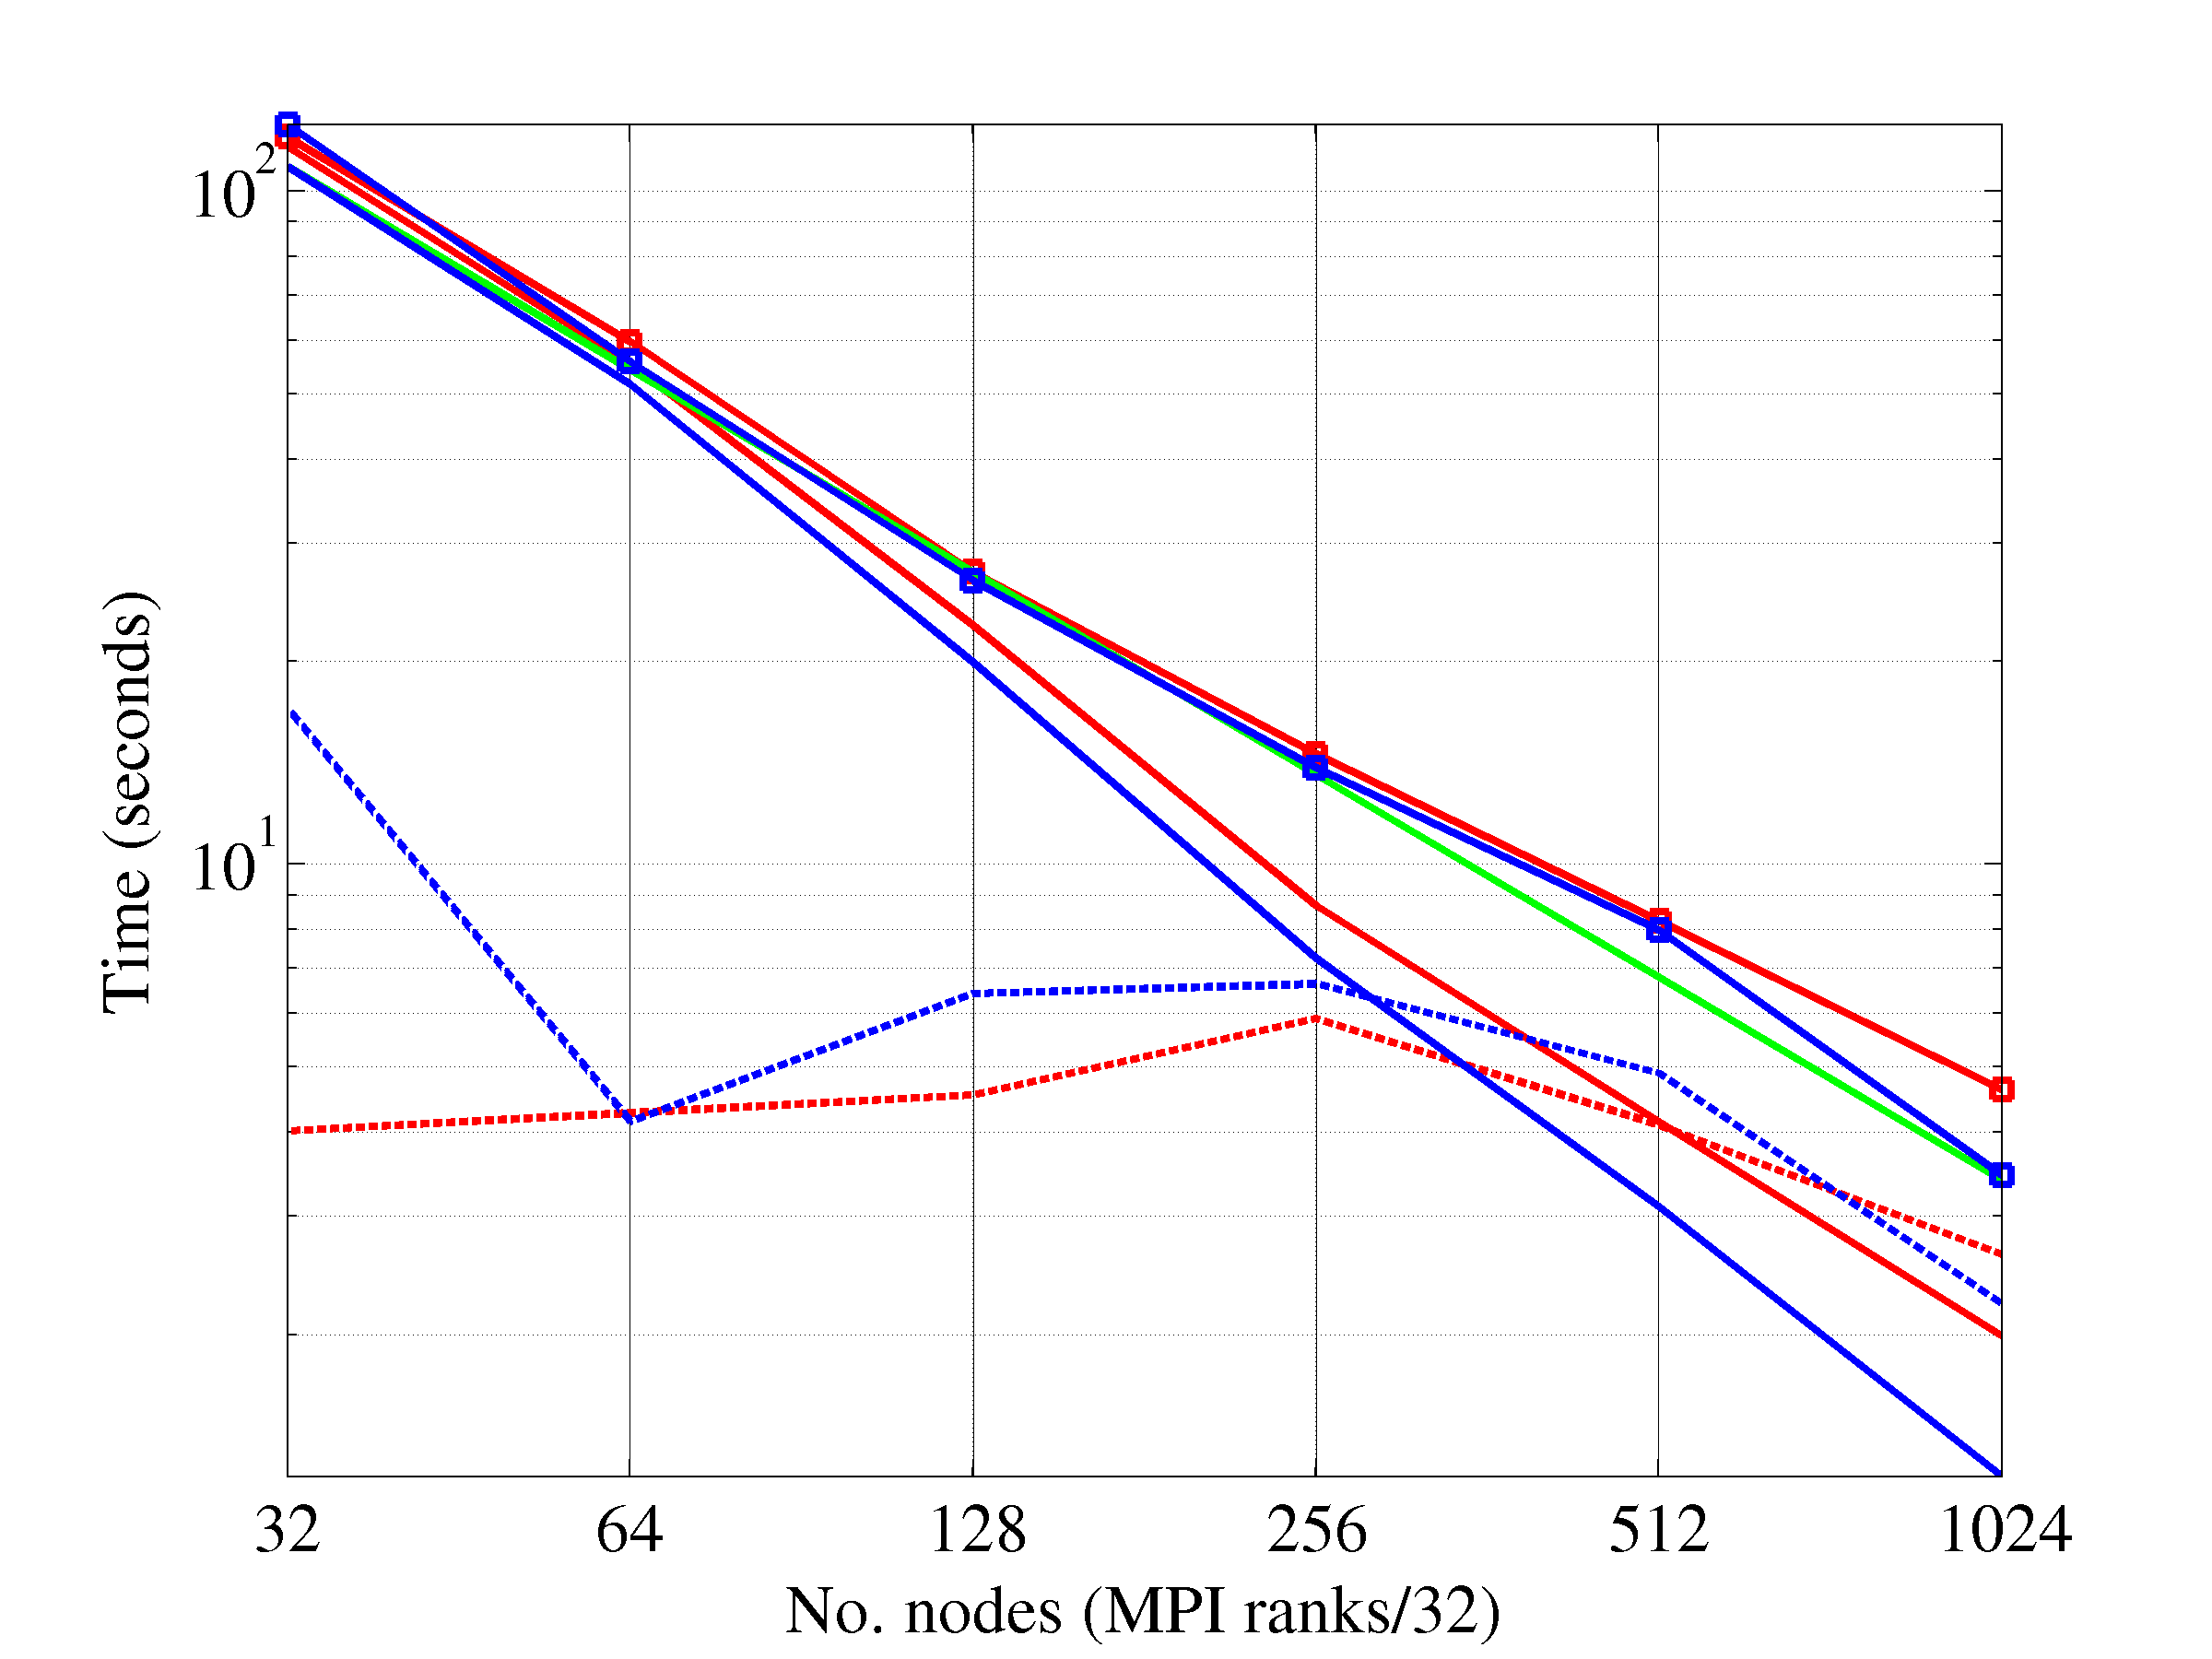
\includegraphics[width=0.7\linewidth]{BeskowReTau550.png}
\end{itemize}

\end{frame}

\section{Procedure}

\begin{frame}{AMG procedure}

\textbf{Current:}
\begin{enumerate}
\item Nek5000 (\textit{IFAMG="true"} and \textit{IFAMG\_DUMP="true"}).
\vspace{3mm}
\item \only<1-2>{Serial Matlab code.} \only<3>{\st{Serial Matlab code.}}
\vspace{3mm}
\item Nek5000 (\textit{IFAMG="true"} and \textit{IFAMG\_DUMP="false"}).
\end{enumerate}

\vspace{4mm}

\onslide<2->{
\textbf{Drawbacks:}
\begin{itemize}
\item Requires Matlab.
\item Serial.
\item External code.
\end{itemize}
}

\vspace{4mm}

\onslide<3->{
\textbf{Future:}
{\color{red} Parallel C} code (Shared memory - Openmp).
}

\end{frame}

\section{C code and parallelization}

\begin{frame}{C code}

\onslide<1->{
\textbf{First step:} rewrite code in serial C.

\vspace{5mm}
}

\onslide<2->{
\textbf{Key points:} 
\begin{itemize}
\item Newer version of the code (\textit{amg\_matlab2}).
\item Matrices under Compressed Sparse Row (CSR) storage.
\item Write Matlab functions in C.
\end{itemize}

\vspace{5mm}
}

\onslide<3->{
\textbf{Status:} 
\begin{itemize}
\item Coarsening and smoothing done.
\item Validated for small test cases.
\item Interpolation under progress.
\end{itemize}
}

\end{frame}

\begin{frame}{Parallelization}

\onslide<1->{
\textbf{First idea:} MPI (distributed memory) via gather-scatter and other communication libraries.

\vspace{3mm}
}

\onslide<2->{
\textbf{Problems:} 
\begin{itemize}
\item Very low number of grid points per core (coarse grid solver).
\item Communication dominated.
\item Complex implementation.
\end{itemize}

\vspace{5mm}
}

\onslide<3->{
\textbf{Solution:} Shared memory and Openmp

\vspace{3mm}
}

\onslide<4->{
\textbf{Advantages:} 
\begin{itemize}
\item No communication.
\item Easier to implement.
\item Significant time reduction still possible on clusters (16, 32, 68... cores).
\end{itemize}
}

\end{frame}

\begin{frame}{Results}

First plot of some kind of scaling ???

\end{frame}

\section{Other projects}

\begin{frame}{Other projects}{Error estimators and Adaptive mesh refinement}
\textbf{Flow past a 2D cylinder:} Velocity magnitude - $Re=100$ - Pol. Order$ = 5$

\centering
  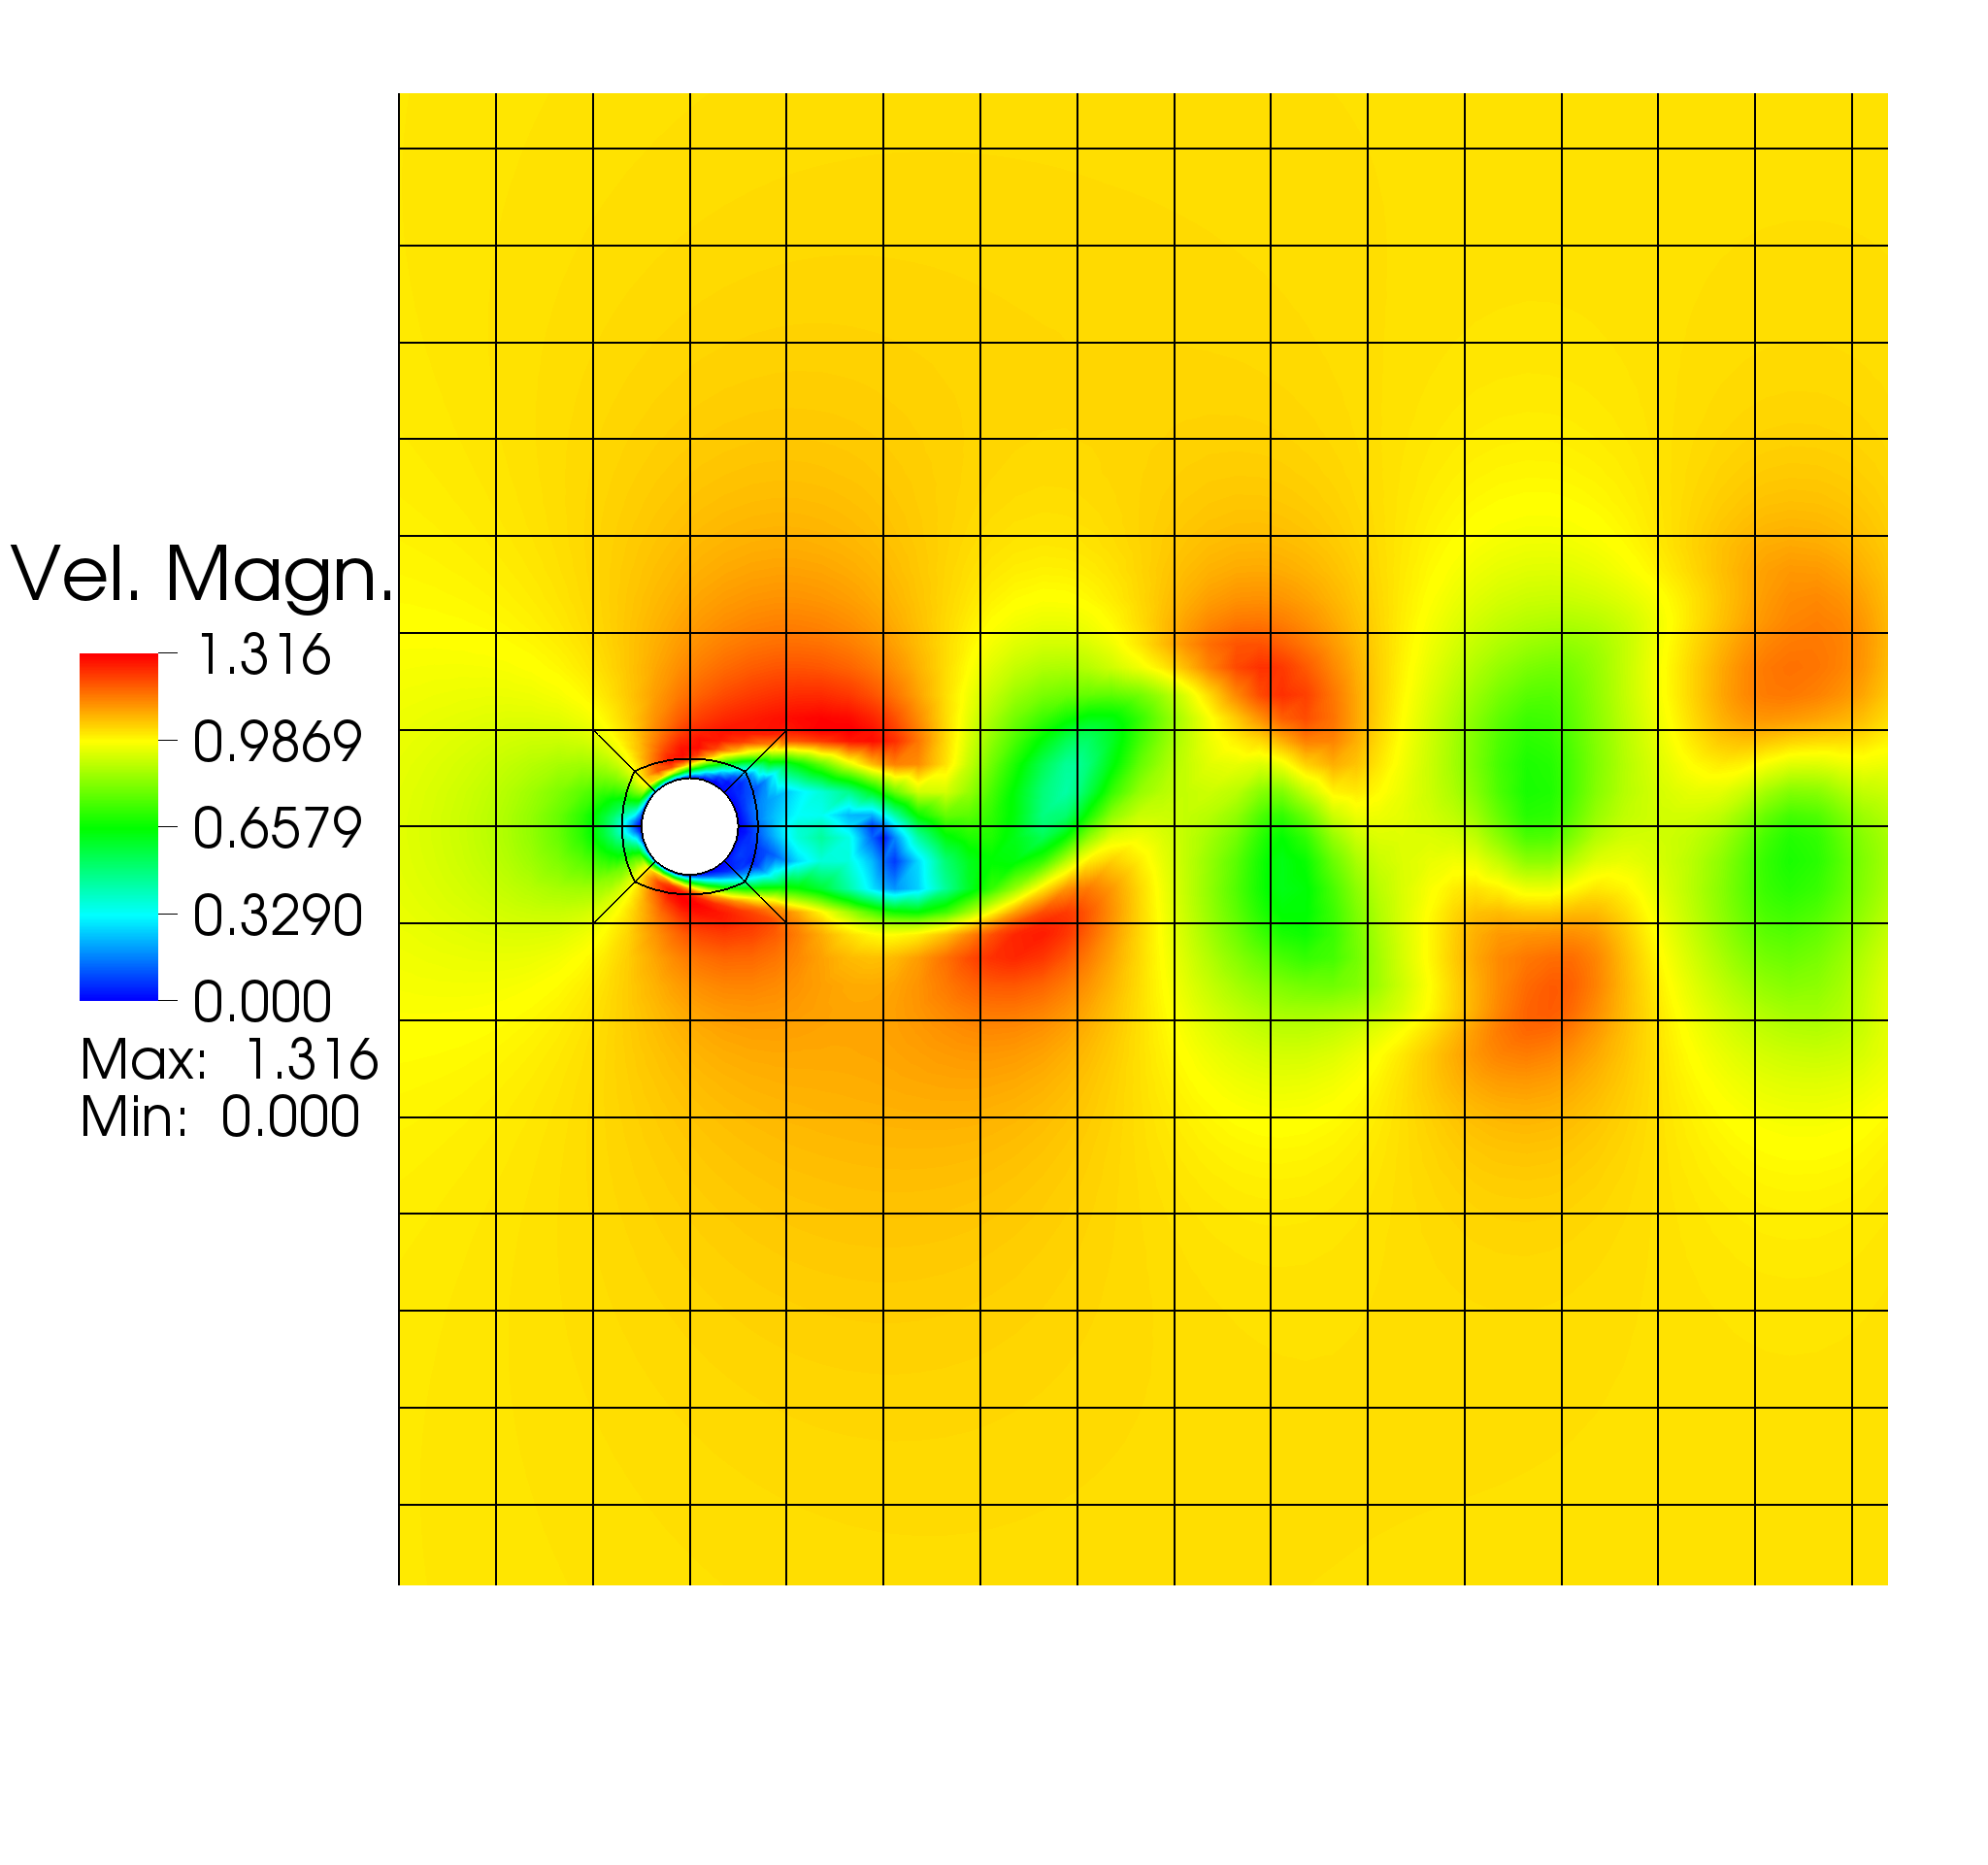
\includegraphics[trim={0 14.5cm 0 7.2cm},clip, width=0.8\linewidth]{vel_init} 
\end{frame}

\begin{frame}{Other projects}{Error estimators and Adaptive mesh refinement}
\textbf{Flow past a 2D cylinder:} Averaged error estimator - $Re=100$ - Pol. Order $= 5$

Error estimators by C. Mavriplis.

\centering
  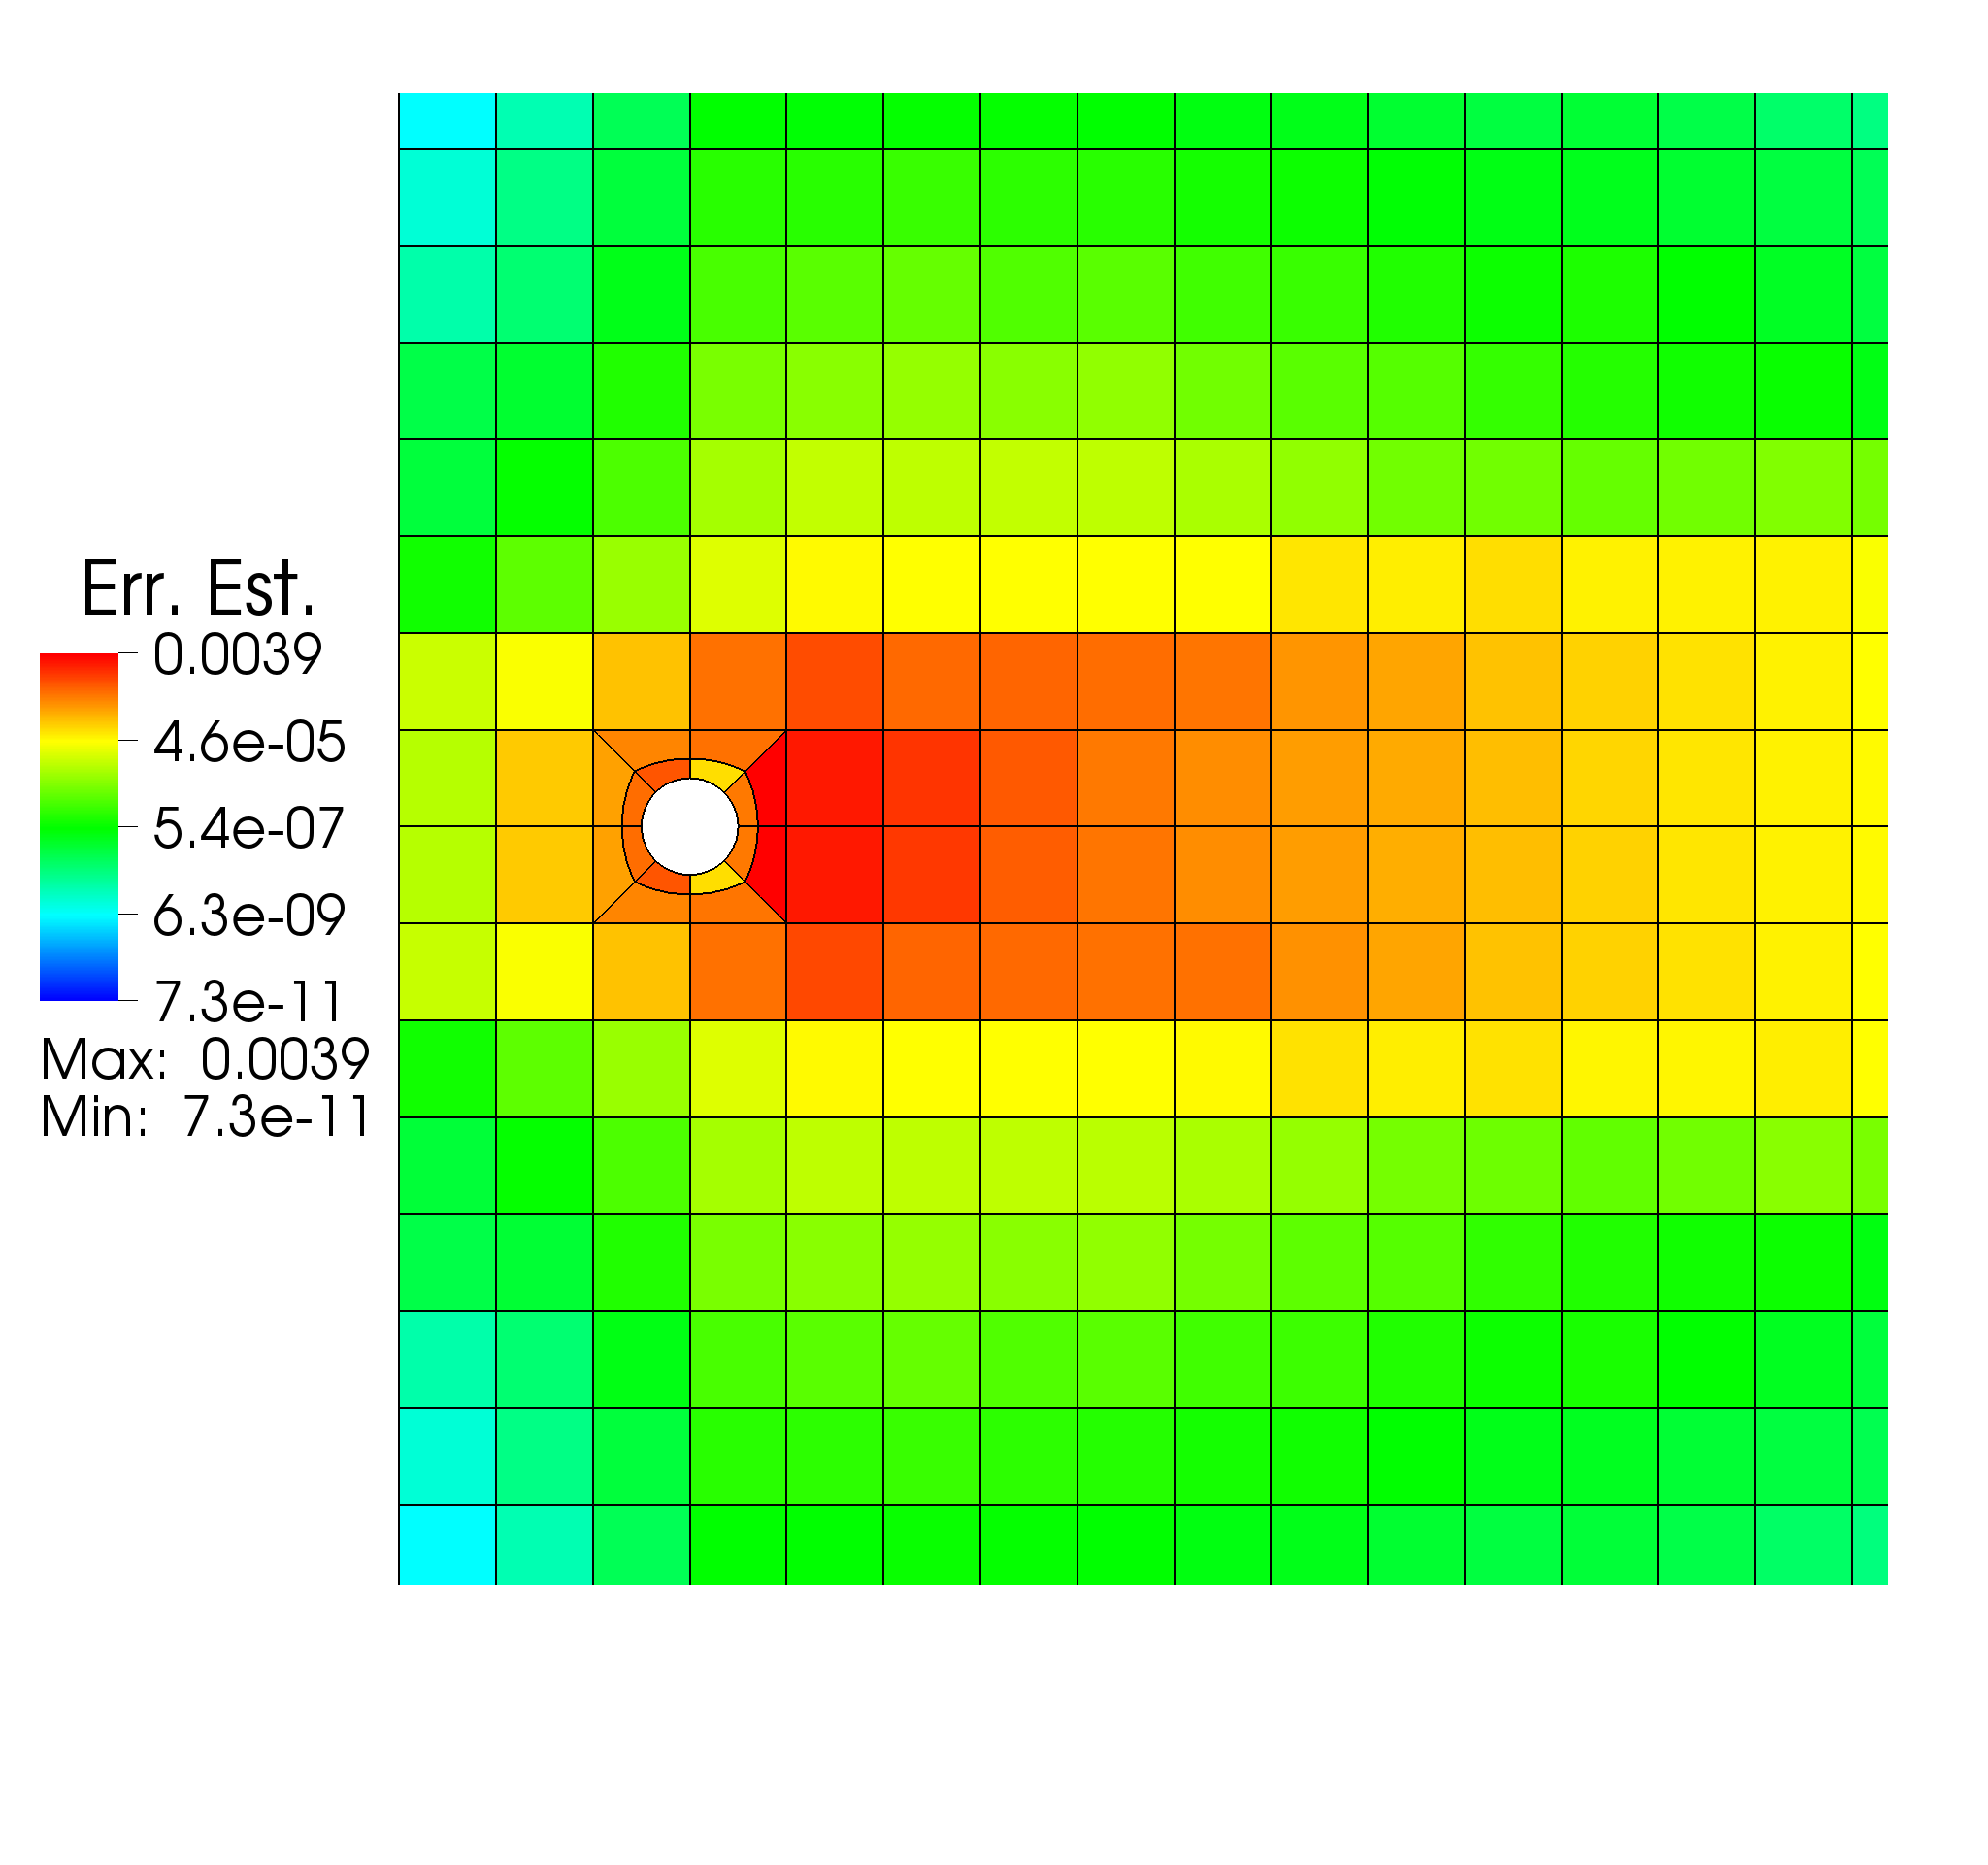
\includegraphics[trim={0 14.5cm 0 7.2cm},clip, width=0.8\linewidth]{err_est} 
\end{frame}

\begin{frame}{Other projects}{Error estimators and Adaptive mesh refinement}
\textbf{Flow past a 2D cylinder:} Velocity magnitude - $Re=100$ - Pol. Order$ = 5$

\centering
  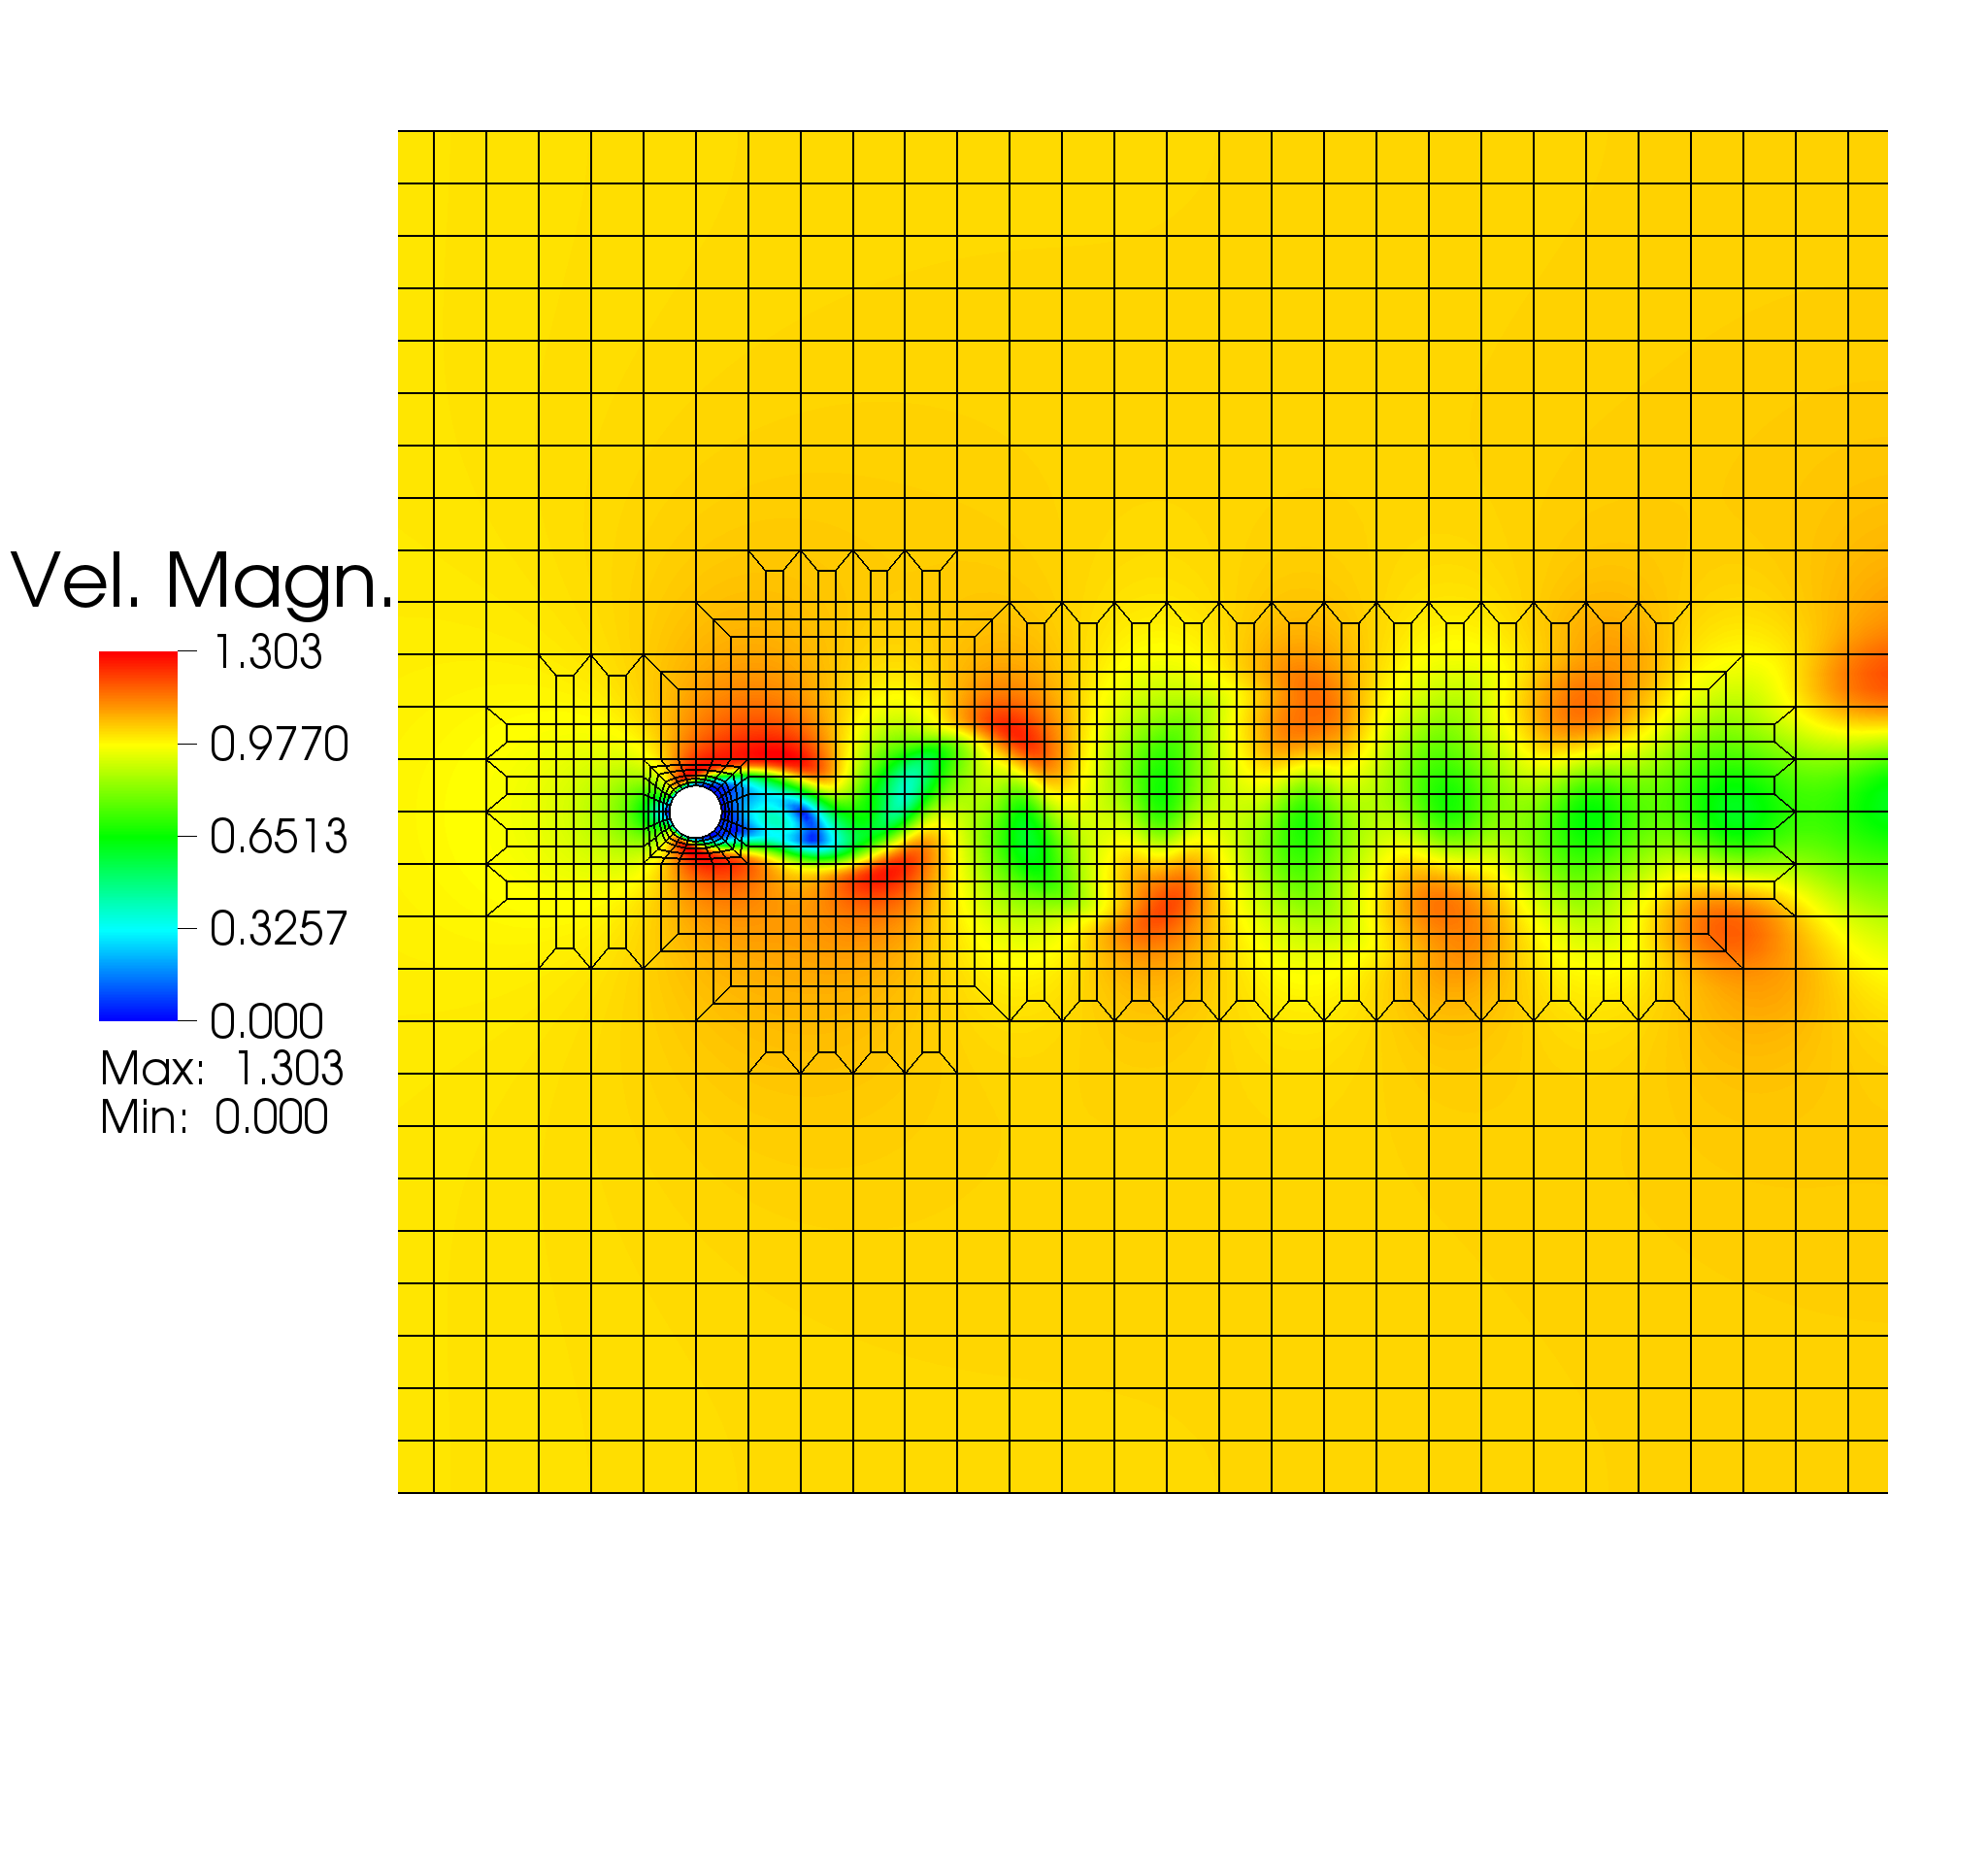
\includegraphics[trim={0 18cm 3cm 10cm},clip, width=0.8\linewidth]{ref_cyl_velmagn} 
\end{frame}

\begin{frame}{Other projects}{P-refinement}

\onslide<1->{
\textbf{Objective:} Variable polynomial order over elements.

\vspace{4mm}
}

\onslide<2->{
\textbf{Status:}
\begin{itemize}
\item Interpolation operator at element boundaries.
\item Gather scatter operator.
\item \textit{axhelm} function implemented.
\end{itemize}

\vspace{4mm}
}

\onslide<3->{
\textbf{Future:}
\begin{itemize}
\item Conjugate gradient solver.
\item Heat equation.
\end{itemize}
}

\end{frame}

\begin{frame}
\Huge{\centerline{The End}}
\end{frame}

%----------------------------------------------------------------------------------------

%\thanksframe \label{final-frame}

\end{document} 